% Generated from audited JSON by generate_2026_09_11_collaborator_slides.py.
% Build: latexmk -pdf -interaction=nonstopmode -halt-on-error THIS_FILE.tex
\documentclass[10pt,aspectratio=169]{beamer}
\usepackage[T1]{fontenc}
\usepackage{lmodern,amsmath,amssymb,booktabs,graphicx}
\definecolor{ink}{HTML}{172B3A}
\definecolor{teal}{HTML}{087E8B}
\definecolor{amber}{HTML}{A85317}
\definecolor{muted}{HTML}{5A6C7B}
\definecolor{pale}{HTML}{EEF5F6}
\definecolor{warm}{HTML}{FBF3E9}
\setbeamercolor{normal text}{fg=ink,bg=white}
\setbeamercolor{structure}{fg=teal}
\setbeamercolor{frametitle}{fg=ink}
\setbeamercolor{block title}{fg=teal,bg=pale}
\setbeamercolor{block body}{fg=ink,bg=pale}
\setbeamercolor{block title alerted}{fg=amber,bg=warm}
\setbeamercolor{block body alerted}{fg=ink,bg=warm}
\setbeamerfont{frametitle}{size=\Large,series=\bfseries}
\setbeamerfont{title}{size=\LARGE,series=\bfseries}
\setbeamertemplate{navigation symbols}{}
\setbeamertemplate{itemize items}[circle]
\setbeamersize{text margin left=8mm,text margin right=8mm}
\setbeamertemplate{frametitle}{\vspace{2mm}\insertframetitle\par\vspace{2mm}}
\setbeamertemplate{footline}{\hspace{8mm}\color{muted}\tiny
NM-ROM $\vert$ Audited development results $\vert$ September 2026\hfill
\insertframenumber/\inserttotalframenumber\hspace{8mm}\vspace{3mm}}
\setlength{\tabcolsep}{4pt}
\renewcommand{\arraystretch}{1.2}
\newcommand{\smallnote}[1]{\par\vspace{1mm}{\scriptsize\color{muted}#1\par}}
\newcommand{\takeaway}[1]{\begin{block}{Takeaway}#1\end{block}}
\newcommand{\caution}[1]{\begin{alertblock}{Interpretation}#1\end{alertblock}}
\title{Separable NM-ROM\\Multiresolution results}
\subtitle{\texorpdfstring{Poisson 2D $\cdot$ Heat 2D $\cdot$ Burgers 2D $\cdot$ Reflective waves}{Poisson 2D; Heat 2D; Burgers 2D; Reflective waves}}
\author{Tunable NM-ROM project}
\date{11 September 2026}
\hypersetup{pdftitle={Separable NM-ROM: multiresolution results},pdfauthor={Tunable NM-ROM project}}
\begin{document}
\begin{frame}{}
\titlepage
\vspace{-4mm}
\begin{center}\small\color{teal}Frozen trained weights across all tested resolutions\end{center}
\smallnote{Paired GPU measurements and independently audited fields. Development cohorts; independent final paper validation remains open.}

\end{frame}

\begin{frame}{At 1024 intervals: where the evidence stands}
\small Fastest tested iterative FOM meeting the declared target, divided by ROM time.\par\vspace{3mm}\par\noindent\begin{tabular*}{\textwidth}{@{\extracolsep{\fill}}lrrl@{}}
\toprule
Problem & FOM/ROM & ROM error \% & ROM status \\ \midrule
Poisson 2D & 33.91 & 6.802 & Accuracy target missed \\
Heat 2D & 4.85 & 4.555 & Target and stopping pass \\
Burgers 2D & 1.63 & 3.908 & Accuracy passes; stalls$^*$ \\
Reflective waves & 0.23 & 3.568 & Full-state target missed \\
\bottomrule\end{tabular*}\par
\takeaway{Heat has the clearest qualified speed advantage. Burgers has a smaller fine-grid advantage under its existing stopping contract.}\smallnote{Ratio above one favors the ROM. These are named iterative controls, not the fastest possible FOMs. Errors are worst cases under the panel-specific norms.}\smallnote{$^*$Burgers accepts small-step/improvement stalls; stationarity was not measured. Reflective-wave error here is displacement only.}
\end{frame}

\begin{frame}{The measurement contract}
\small
\begin{itemize}
\item Meshes: $N=64, 256, 1024$ intervals per axis. One frozen checkpoint per PDE/boundary.
\item Online GPU time includes input projection/fitting, the solve or rollout, and requested full fields.
\item Training, mesh assembly and compilation are offline. Host transfers are reported separately.
\item Each ROM/FOM comparison uses one GPU allocation; costs and errors come from the same invocation.
\end{itemize}\vspace{2mm}
\par\noindent\begin{tabular*}{\textwidth}{@{\extracolsep{\fill}}lrrl@{}}
\toprule
Problem & Cases & Repeats & Error normalization \\ \midrule
Poisson 2D & 30 & 3 & Current solution norm \\
Heat 2D & 12 & 3 & Current field norm \\
Burgers 2D & 4 & 3 & Fixed initial field norm \\
Reflective waves & 2 & 3 & Current component norms \\
\bottomrule\end{tabular*}\par

\smallnote{Times: medians of all retained repetitions, with equal repeats per case. Errors: maxima over cases, output times and repetitions. All repetitions and outliers are retained.}
\smallnote{The target is 5\%, with panel-specific refinement and solver checks. Wave qualification includes displacement, velocity and energy state.}

\end{frame}

\begin{frame}{Shared decoder; explicitly named full solvers}

\vspace{-2mm}\[u(x;z)=\sum_{j=1}^{R} g_j(x)\,h_j(z),\qquad u=G\,h(z).\]
\small The spatial bank is fixed during a query. The nonlinear coefficient map is evaluated as latent coordinates change.
\vspace{2mm}
\par\noindent\begin{tabular*}{\textwidth}{@{\extracolsep{\fill}}lll@{}}
\toprule
Problem & Reduced computation & Primary iterative FOM \\ \midrule
Poisson & Preassembled weak algebra & CG: $10^{-6}$ \\
Heat & Weak CN; Cholesky updates & CN--CG: $10^{-6}$ \\
Burgers & Preassembled linear; sampled upwind & Newton $10^{-6}$; linear $10^{-8}$ \\
Reflective waves & Nonlinear projected RK4 dynamics & Midpoint CG: $10^{-6}$ \\
\bottomrule\end{tabular*}\par
\smallnote{CG = conjugate gradient; CN = Crank--Nicolson. Burgers uses FFT-preconditioned Newton--BiCGStab. Weak equations average the residual against smooth tests.}\smallnote{\textbf{Scope:} Burgers uses sampled sign-upwind advection, not the historical polynomial tensor. Wave ROM/FOM use the same step size with different integration formulas.}
\end{frame}

\begin{frame}{ROM runtime stays nearly flat over these meshes}

\begin{center}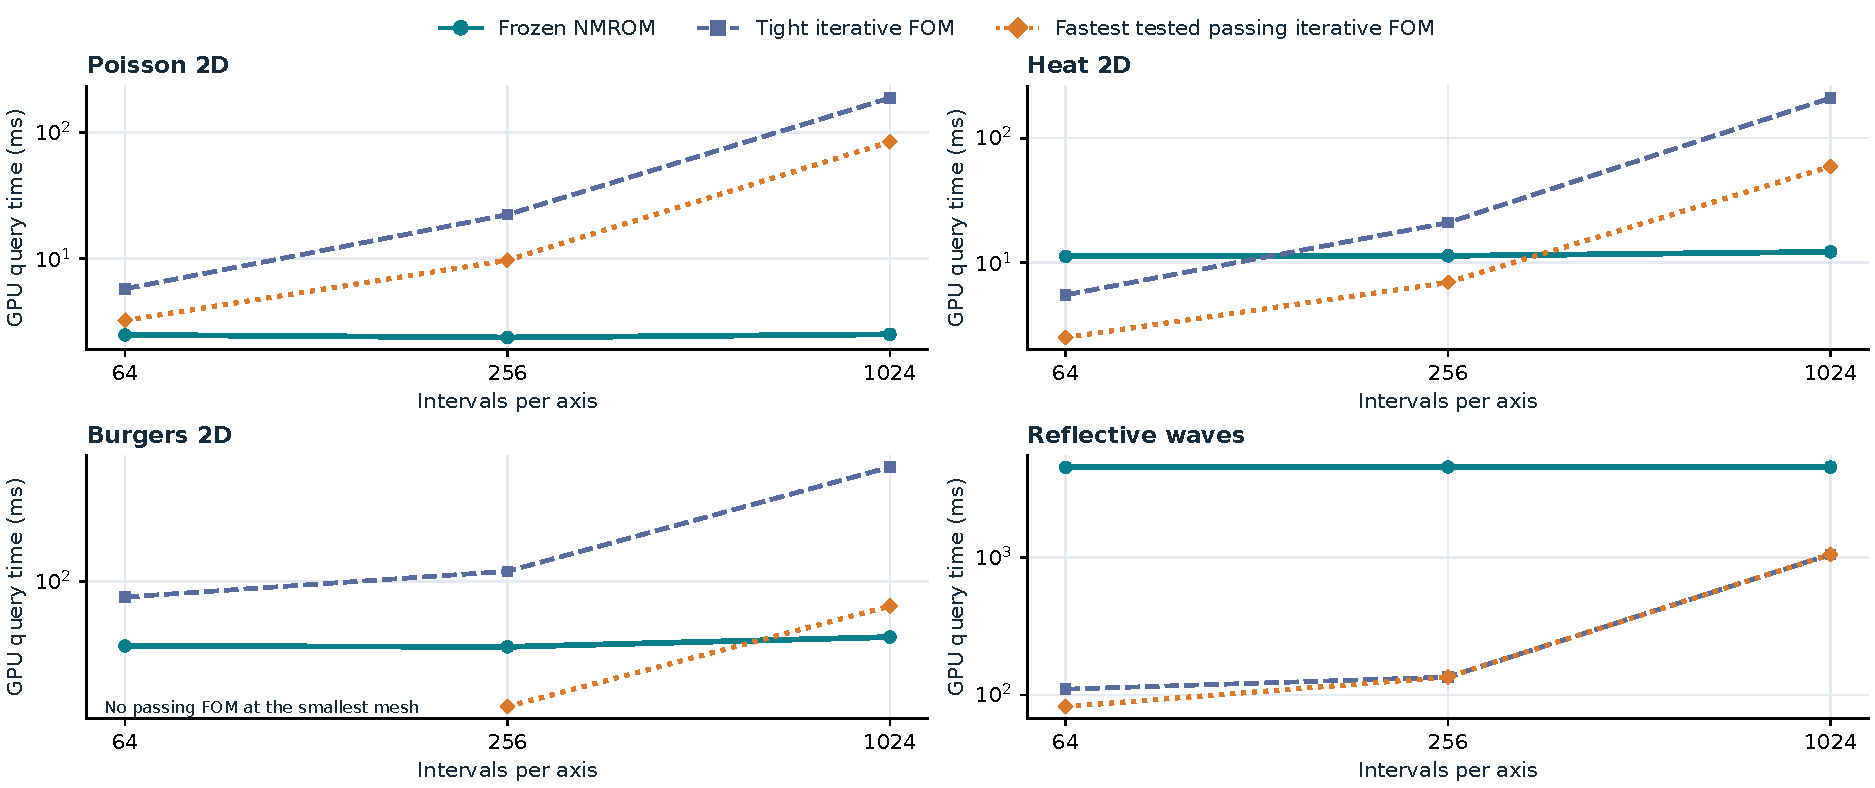
\includegraphics[width=.97\textwidth,height=.63\textheight,keepaspectratio]{2026-09-11-multiresolution-collaborator-slides-figures/runtime-scaling.pdf}\end{center}
\smallnote{Logarithmic axes. Orange: fastest tested iterative FOM satisfying the declared target at that mesh. A faster ROM curve alone does not establish an accuracy-qualified win.}
\smallnote{This is a finite-range observation. Reading dense inputs and producing full fields still depend on mesh size. Compare methods within each panel, not across different GPU allocations.}

\end{frame}

\begin{frame}{Poisson: strong runtime scaling; accuracy needs work}
\small Primary FOM: zero-start, unpreconditioned CG at $10^{-6}$.\par\vspace{2mm}\par\noindent\begin{tabular*}{\textwidth}{@{\extracolsep{\fill}}lrrrrr@{}}
\toprule
$N$ & ROM ms & FOM ms & FOM/ROM & ROM error \% & FOM error \% \\ \midrule
64 & 2.47 & 5.73 & 2.32 & 6.803 & 0.2572 \\
256 & 2.36 & 22.28 & 9.46 & 6.802 & 0.01546 \\
1024 & 2.49 & 188.21 & 75.45 & 6.802 & 0.0007351 \\
\bottomrule\end{tabular*}\par
\vspace{2mm}\takeaway{The decoder transfers across meshes with nearly unchanged error and runtime. Its worst error remains above the 5\% target.}
\small At $N=1024$, loose CG at $10^{-1}$ takes 84.58 ms with 1.019\% error. The raw FOM/ROM ratio is 33.91, but the ROM fails the target.
\smallnote{Error: current-relative solution $L_2$, against a refined finite-difference reference. Reference allowance is included in qualification. All recorded ROM solves satisfy stationarity and all CG controls converge.}

\end{frame}

\begin{frame}{Heat: a fine-grid speedup that survives looser CG}
\small Primary FOM: matched Crank--Nicolson steps, CG at $10^{-6}$.\par\vspace{2mm}\par\noindent\begin{tabular*}{\textwidth}{@{\extracolsep{\fill}}lrrrrr@{}}
\toprule
$N$ & ROM ms & FOM ms & FOM/ROM & ROM error \% & FOM error \% \\ \midrule
64 & 11.23 & 5.51 & 0.490 & 4.559 & 0.06738 \\
256 & 11.34 & 21.00 & 1.85 & 4.556 & 0.03126 \\
1024 & 12.21 & 210.60 & 17.25 & 4.555 & 0.03491 \\
\bottomrule\end{tabular*}\par
\vspace{2mm}\takeaway{At $N=1024$, the ROM remains 4.85$\times$ faster than the fastest tested passing iterative FOM. Both satisfy the physical target and stopping checks.}
\small Looser CG at $10^{-2}$: 59.18 ms and 0.7707\% error. Including input/output transfers, the FOM/ROM ratio is 2.27.
\smallnote{Error: current-relative field $L_2$, against a refined continuum sine-series solution. Coarse-grid CG remains faster; the medium-grid advantage depends on tolerance.}

\end{frame}

\begin{frame}{Burgers: fine-grid gain with stalled solves}
\small Primary FOM: FFT-preconditioned Newton--BiCGStab, $10^{-6}/10^{-8}$.\par\vspace{2mm}\par\noindent\begin{tabular*}{\textwidth}{@{\extracolsep{\fill}}lrrrrr@{}}
\toprule
$N$ & ROM ms & FOM ms & FOM/ROM & ROM error \% & FOM error \% \\ \midrule
64 & 36.23 & 78.24 & 2.16 & 10.85 & 10.99 \\
256 & 35.75 & 117.47 & 3.29 & 4.551 & 4.027 \\
1024 & 41.68 & 605.75 & 14.53 & 3.908 & 2.142 \\
\bottomrule\end{tabular*}\par
\vspace{2mm}\takeaway{At $N=1024$: 1.63$\times$ faster than the fastest tested passing iterative FOM. The two larger ROM meshes pass the physical target.}
\small Looser FOM: Newton $10^{-2}$, linear $5\times10^{-1}$; 68.04 ms, 2.39\% error. With transfers: 1.44$\times$.
\smallnote{\textbf{Stopping limitation:} all ROM fits/steps stop by a small-step/improvement rule; stationarity is unmeasured. Both ROM and FOM miss the physical target on the smallest mesh.}
\smallnote{Error uses the fixed initial reference norm. Spatial/temporal reference allowances are included in the physical gate.}

\end{frame}

\begin{frame}{Reflective waves: displacement alone is incomplete}
\small Primary FOM: implicit-midpoint CG at $10^{-6}$.\par\vspace{2mm}\par\noindent\begin{tabular*}{\textwidth}{@{\extracolsep{\fill}}lrrrrr@{}}
\toprule
$N$ & ROM ms & FOM ms & FOM/ROM & ROM error \% & FOM error \% \\ \midrule
64 & 4510.12 & 110.53 & 0.025 & 3.641 & 0.3521 \\
256 & 4530.34 & 135.46 & 0.030 & 3.569 & 0.3534 \\
1024 & 4532.59 & 1053.34 & 0.232 & 3.568 & 0.3532 \\
\bottomrule\end{tabular*}\par
\vspace{1mm}\begin{columns}[T]
\column{.47\textwidth}\small
At $N=1024$: current-relative errors.
\par\noindent\begin{tabular*}{\textwidth}{@{\extracolsep{\fill}}lrr@{}}
\toprule
Component & ROM \% & FOM \% \\ \midrule
Displacement & 3.568 & 0.353 \\
Velocity & 7.813 & 0.790 \\
Energy state & 6.214 & 0.608 \\
\bottomrule\end{tabular*}\par

\column{.49\textwidth}\small
\caution{The ROM is slower at every mesh. Displacement meets the descriptive target, but velocity and energy state do not.}
\end{columns}
\smallnote{Reference: the exact modal solution of the same spatial discretization. These are not continuum error bounds. Full host-to-host wave timing was not measured.}

\end{frame}

\begin{frame}{The FOM algorithm and tolerance change the conclusion}
\small At $N=1024$: all entries below are FOM/ROM runtime ratios.
\vspace{2mm}\par\noindent\begin{tabular*}{\textwidth}{@{\extracolsep{\fill}}lrrr@{}}
\toprule
Problem & Tight iterative & Fastest passing & Passing + transfers \\ \midrule
Poisson 2D & 75.45 & 33.91 & 14.90 \\
Heat 2D & 17.25 & 4.85 & 2.27 \\
Burgers 2D & 14.53 & 1.63 & 1.44 \\
Reflective waves & 0.23 & 0.23 & Not measured \\
\bottomrule\end{tabular*}\par

\vspace{2mm}\begin{columns}[T]
\column{.47\textwidth}\small
Direct sine-transform diagnostics:
\par\noindent\begin{tabular*}{\textwidth}{@{\extracolsep{\fill}}lrr@{}}
\toprule
Problem & GPU ms & Error \% \\ \midrule
Poisson 2D & 0.317 & 0.0007351 \\
Heat 2D & 1.236 & 0.0003501 \\
Reflective waves & 16.624 & 0 \\
\bottomrule\end{tabular*}\par

\column{.49\textwidth}\small
\caution{Specialized direct solvers are faster on these separable linear problems. Iterative-FOM wins do not establish a universal FOM advantage.}
\end{columns}
\smallnote{Loose controls are selected on development cases; they are not globally optimal classical solvers. Poisson still misses the ROM target; Burgers retains its stall qualification. Wave direct displacement error is zero against the same-grid modal reference.}

\end{frame}

\begin{frame}{Reflective-wave cost is in latent evolution}
\begin{columns}[T]
\column{.47\textwidth}\small
At $N=1024$:
\par\noindent\begin{tabular*}{\textwidth}{@{\extracolsep{\fill}}lr@{}}
\toprule
Component & GPU ms \\ \midrule
Initialization and projection & 20.18 \\
Latent evolution & 4510.05 \\
Dense GPU output & 2.51 \\
\bottomrule\end{tabular*}\par

\takeaway{99.50\% of query time is spent in latent evolution.}
\column{.49\textwidth}\small
$T=2.4$, $\Delta t=0.0025$:
\[ 960\text{ steps}\times4 = 3840\text{ RK stages}. \]
At every stage:
\begin{itemize}
\item Decoder Jacobian and directional curvature.
\item QR factorization and triangular solve.
\item SVD check of tangent rank.
\end{itemize}
\end{columns}
\caution{The stage loop is fully reduced, but repeats expensive state-dependent work. Individual derivative, QR, SVD and GPU execution costs have not yet been separated.}
\smallnote{Component medians need not sum exactly to the total median. One additional initial acceleration/rank check precedes the RK stages. Proposed next step: profile stage operations, then test cheaper guarding and fewer stages with accuracy checks.}

\end{frame}

\begin{frame}{What we can show now; what needs improvement}

\small
\begin{columns}[T]
\column{.48\textwidth}
\begin{block}{Supported by this development study}
\begin{itemize}
\item Fixed learned weights transfer across the tested meshes.
\item Reduced query time is nearly flat over this range.
\item Heat beats the tested iterative FOM frontier on the finest mesh.
\item Burgers has a smaller fine-grid gain with an explicit stopping limitation.
\end{itemize}
\end{block}
\column{.48\textwidth}
\begin{alertblock}{Next experiments, not current results}
\begin{itemize}
\item Poisson: reduce physical error and diagnose representation versus projection limits.
\item Burgers: measure stationarity and improve coarse-grid accuracy.
\item Reflective waves: reduce stage cost; improve velocity and energy accuracy.
\item Freeze choices, then evaluate independent final cases and training seeds.
\end{itemize}
\end{alertblock}
\end{columns}
\smallnote{A tunability claim requires an additional fixed-checkpoint physical-error versus cost study. Adjustable tolerances alone do not establish that tradeoff.}

\end{frame}

\begin{frame}{Proposed: tunability from one trained network}

\small
Train once per PDE, then select an inference configuration with unchanged weights.
\vspace{2mm}
\begin{tabular*}{\textwidth}{@{\extracolsep{\fill}}lll@{}}
\toprule
Knob & Intended cost change & Current status \\ \midrule
Active latent coordinates $k$ & Smaller derivatives and solves & Subset accuracy unvalidated \\
Active spatial bank size $R$ & Smaller operators and output map & Subset accuracy unvalidated \\
Solver budget / tolerance & Fewer or more corrections & Available with frozen weights \\
Time step $\Delta t$ & Fewer or more evolution steps & Available for time-dependent PDEs \\
\bottomrule
\end{tabular*}
\vspace{2mm}
\[
u_{\ell}(x)=\sum_{j=1}^{R_{\ell}}g_j(x)\,
h_{\ell,j}(z_1,\ldots,z_{k_{\ell}}).
\]
\small Train shared weights with a loss at every supported level $\ell$. At inference,
choose a level and solver budget; physically omit inactive computation.
\smallnote{\textbf{Proposed, not measured:} screen truncation of current checkpoints as an ablation; train shared capacity levels if it is unreliable. Zero masks alone may not save runtime.}

\end{frame}

\begin{frame}{Proposed: demonstrate a physical accuracy--cost curve}

\small
\begin{columns}[T]
\column{.48\textwidth}
\begin{block}{First: current frozen checkpoints}
\begin{itemize}
\item Sweep solve budgets/tolerances at fixed capacity; time steps separately.
\item Pair physical error and full-query time; retain stopping failures.
\item Find where additional computation stops improving physical accuracy.
\end{itemize}
\end{block}
\column{.48\textwidth}
\begin{block}{Then: shared capacity levels}
\begin{itemize}
\item Train with losses at each $(k_{\ell},R_{\ell})$; preassemble each level's operators.
\item Keep more weak equations than latent coordinates; validate each budget.
\item Freeze choices, then compare with passing FOMs on independent cases.
\end{itemize}
\end{block}
\end{columns}
\caution{Lower weak residual need not mean lower physical error. A tolerance setting does not guarantee a requested accuracy, and iterations cannot remove every representation limit.}
\smallnote{Proposed figure: physical error versus query time, one curve per checkpoint; retain failures and all configurations. Select useful operating points on validation cases. This has not been demonstrated by the mesh-scaling tables.}

\end{frame}

\begin{frame}{Audit trail and development limitations}
\small\par\noindent\begin{tabular*}{\textwidth}{@{\extracolsep{\fill}}llll@{}}
\toprule
Panel & Job & GPU & Scientific source \\ \midrule
Poisson 2D & 3534456 & A100 80 GB & \texttt{085e318} \\
Heat 2D & 3529772 & A100 40 GB & \texttt{7e6d2e3} \\
Burgers 2D & 3534502 & A100 40 GB & \texttt{46ced2f} \\
Reflective waves & 3534457 & A100 80 GB & \texttt{e1d3779} \\
\bottomrule\end{tabular*}\par
\vspace{2mm}\begin{columns}[T]\column{.47\textwidth}\small GPU outliers, ascending mesh order:\par\par\noindent\begin{tabular*}{\textwidth}{@{\extracolsep{\fill}}lrr@{}}
\toprule
Panel & ROM & Tight FOM \\ \midrule
Poisson 2D & 2/1/1 & 0/0/0 \\
Heat 2D & 0/0/0 & 0/0/0 \\
Burgers 2D & 0/0/0 & 0/0/0 \\
Reflective waves & 0/0/0 & 0/0/0 \\
\bottomrule\end{tabular*}\par
\column{.49\textwidth}\footnotesize\begin{itemize}\item GPU, float64 and highest precision verified; burn-in before timing.\item Paired full fields and repetition arrays retained; no outlier exclusions.\item Source/reference/field audits passed; archives checksum-verified.\item Final paper cases remain unopened.\end{itemize}\end{columns}\smallnote{Audit success does not imply physical accuracy or stationarity. Exact outlier rules and all controls are in the native audits and accompanying report/JSON.}
\end{frame}

\begin{frame}{Glossary: reading the tables and method}

\footnotesize
\begin{columns}[T]
\column{.48\textwidth}
\textbf{NMROM / FOM:} nonlinear-manifold reduced model / solver on the full spatial grid.\par\smallskip
\textbf{$N$, mesh, intervals/axis:} spatial cells along one coordinate; stored-node counts depend on boundaries.\par\smallskip
\textbf{GPU ms / transfers:} online device time in milliseconds / movement of supplied inputs and requested outputs between CPU and GPU.\par\smallskip
\textbf{FOM/ROM:} ratio of median times; above one means the ROM is faster for that named comparator.\par\smallskip
\textbf{Worst error:} largest normalized field error across cases, output times and repetitions. Current-relative uses the reference norm at that time; fixed-initial uses its initial norm.\par\smallskip
\textbf{Target / refinement:} physical-error threshold with numerical checks / disagreement after refining the reference or time step.
\column{.48\textwidth}
\textbf{Frozen checkpoint / development cases:} unchanged trained weights / already opened inputs used while developing the method.\par\smallskip
\textbf{Bank, $G$, $R$, head, $z$:} learned spatial shapes, their grid matrix and count, nonlinear mixing map, and unknown latent coordinates.\par\smallskip
\textbf{Weak form / residual:} averaging the PDE mismatch against smooth test functions / the mismatch in the solved equations.\par\smallskip
\textbf{CG / BiCGStab / Newton:} iterative linear solvers / successive linearized corrections to nonlinear equations.\par\smallskip
\textbf{CN / midpoint / RK4:} Crank--Nicolson / implicit midpoint / fourth-order Runge--Kutta time integration.\par\smallskip
\textbf{Stationarity / stall:} small objective gradient / small progress or step, which need not imply stationarity.
\end{columns}

\end{frame}

\begin{frame}{Glossary: operators, numerical work and evidence}

\footnotesize
\begin{columns}[T]
\column{.48\textwidth}
\textbf{Preassembly / cached algebra:} forming small operators before each online query and reusing them. Dense input/output work is still mesh-dependent.\par\smallskip
\textbf{Quadrature / sampled upwind:} weighted spatial samples / evaluating the flow-direction-dependent difference operator at those samples.\par\smallskip
\textbf{Tensor:} a multidimensional coefficient array encoding an operator; current Burgers is not the historical polynomial-tensor implementation.\par\smallskip
\textbf{FFT / sine transform / modal solution:} transform algorithms that diagonalize these separable linear problems.\par\smallskip
\textbf{Preconditioning / Cholesky:} making an iterative system easier to solve / a symmetric positive-definite matrix factorization.
\column{.48\textwidth}
\textbf{Jacobian / curvature:} how decoder output changes with latent coordinates / its directional second derivative.\par\smallskip
\textbf{QR / SVD / tangent rank:} matrix factorizations used for least squares and singular values / the number of independent decoder directions.\par\smallskip
\textbf{Energy-state error:} wave error measured jointly through velocity and displacement gradients; it is not merely the difference in total scalar energy.\par\smallskip
\textbf{Median / repetition / outlier:} middle timing value / rerunning one input / an unusually slow repetition under the recorded rule. Repetitions are not independent physical cases.\par\smallskip
\textbf{Tunability / independent final validation:} choosing inference effort at fixed weights / testing frozen choices on previously unopened cases.\par\smallskip
\textbf{Nested levels / masks / nondominated points:} shared weights at several capacities / inactive terms / settings unbeaten in both cost and error.
\end{columns}

\end{frame}

\end{document}
